\documentclass[../cheatSheetAlgoritmi.tex]{subfiles}
\begin{document}

\subsection{Esame 07/02/2019}
\textbf{Le croci} \\
Si consideri una matrice binaria $M$ di dimensione $n \times n$. Scrivere un algoritmo
\begin{center}
\textbf{int} cross(\textbf{int}[ ][ ] M,\textbf{int} n)
\end{center}
che restituisca la dimensione della più grande croce composta da valori $1$ presente nella matrice. Una croce è compostada un bit $1$ centrale e quattro braccia di uguale lunghezza,contenenti bit $1$. Non deve essere necessariamente circondata da bit $0$. \\
Per esempio, la croce visibile nell’esempio è composta da 17 valori 1e l’algoritmo dovrà restituire 17.
\begin{center}
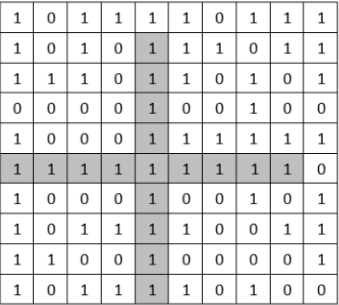
\includegraphics{ ../img/esame_07022019}
\end{center}
\textbf{Soluzione} \\
Il docente propone un approccio basato su programmazione dinamica per risolvere il seguente problema. \\ Si costruiscono quattro matrici di appoggio, chiamate $L,R,U,D$ (left, right, up,down). \\
Le caselle $L[i][j]$, $R[i][j]$, $U[i][j]$, $D[i][j]$ contiene la più lunga fila di valori $1$ che si estende a partire dalla cella $(i, j)$(compresa) nella direzione sinistra, destra, alto, basso. \\
Tali vettori vengono calcolati come segue: 
\begin{equation*}
  	L[i][j] =\begin{cases}
    	M[i][j] & \text{$j = 1$}\\
    	L[i][j-1] + 1 & \text{$j > 1$ \textbf{and} $M[i][j] = 1$}\\
    	0 & \text{$j > 1$ \textbf{and} $M[i][j] = 0$}
  	\end{cases}
\end{equation*}
\begin{equation*}
  	R[i][j] =\begin{cases}
    	M[i][j] & \text{$j = n$}\\
    	R[i][j+1] + 1 & \text{$j < n$ \textbf{and} $M[i][j] = 1$}\\
    	0 & \text{$j < n$ \textbf{and} $M[i][j] = 0$}
  	\end{cases}
\end{equation*}
\begin{equation*}
  	D[i][j] =\begin{cases}
    	M[i][j] & \text{$i = 1$}\\
    	D[i+1][j] + 1 & \text{$i < n$ \textbf{and} $M[i][j] = 1$}\\
    	0 & \text{$i < n$ \textbf{and} $M[i][j] = 0$}
  	\end{cases}
\end{equation*}
\begin{equation*}
  	U[i][j] =\begin{cases}
    	M[i][j] & \text{$i = 1$}\\
    	U[i-1][j] + 1 & \text{$i > 1$ \textbf{and} $M[i][j] = 1$}\\
    	0 & \text{$i > 1$ \textbf{and} $M[i][j] = 0$}
  	\end{cases}
\end{equation*}
Ovvero partendo dalla posizione $(i, j)$ si considerano le somme di 1 sulla rispettiva dimensione, nella cella considerata precedentemente, solo se il valore sulla matrice originale $M$ è 1. \\
Una volta calcolati questi valori è possibile trovare la più grande croce il cui centro è collocato in $(i, j)$ semplicemente calcolando: 
\begin{center}
$min(L[i][j], R[i][j], U[i][j], D[i][j]) \cdot 4 - 3$
\end{center}
Ovvero si usa la più lunga sequenza di valori $1$ consecutiva nelle quattro direzioni possibili e si usa il minimo di questi valori in quanto limita la dimensione della nostra croce. A questo punto, ora che conosciamo il lato della croce più grande possibile centrata in $(i, j)$, calcoliamo in numero di celle che la compongono moltiplicando la dimensione del braccio per 4 e sottraendo 3. Si sottrae 3 dato che in tutte definizioni di $L[i][j], R[i][j], U[i][j]$ e $D[i][j]$ la cella (i, j) è compresa, ed è necessario considerarla una singola volta.
\begin{lstlisting}[ caption = Croce massimale formata da sequenze di 1]
int cross(int[][] M, int n)
	int[][] L = new int[1...n][1...n]
	int[][] R = new int[1...n][1...n]
	int[][] U = new int[1...n][1...n]
	int[][] D = new int[1...n][1...n]
	for j = 1 to n do
		U[1][j] = M[1][j]
		D[n][j] = M[n][j]
	for i = 1 to n do
		L[i][1] = M[i][1]
		R[i][n] = M[i][n]
	for i = 2 to n do
		for j = 2 to n do
			L[i][j] = iif(M[i][j] $==$ 0, 0, L[i][j-1] + 1)
			U[i][j] = iif(M[i][j] $==$ 0, 0, U[i-1][j] + 1)
	for i = n - 1 downto 1 do
		for j = n - 1 downto 1 do
			R[i][j] = iif(M[i][j] $==$ 0, 0, R[i][j+1] + 1)
			D[i][j] = iif(M[i][j] $==$ 0, 0, D[i+1][j] + 1)
	int maxSoFar = 0
	for i = 1 to n do
		for j = 1 to n do
			int size = min(L[i][j], R[i][j], U[i][j], D[i][j]) $\cdot$ 4 - 3
			maxSoFar = max(maxSoFar, size)
	return maxSoFar
\end{lstlisting}
Come è facilmente intuibile, il costo computazionale di tale procedura è di $\Theta(n^2)$.
\end{document}